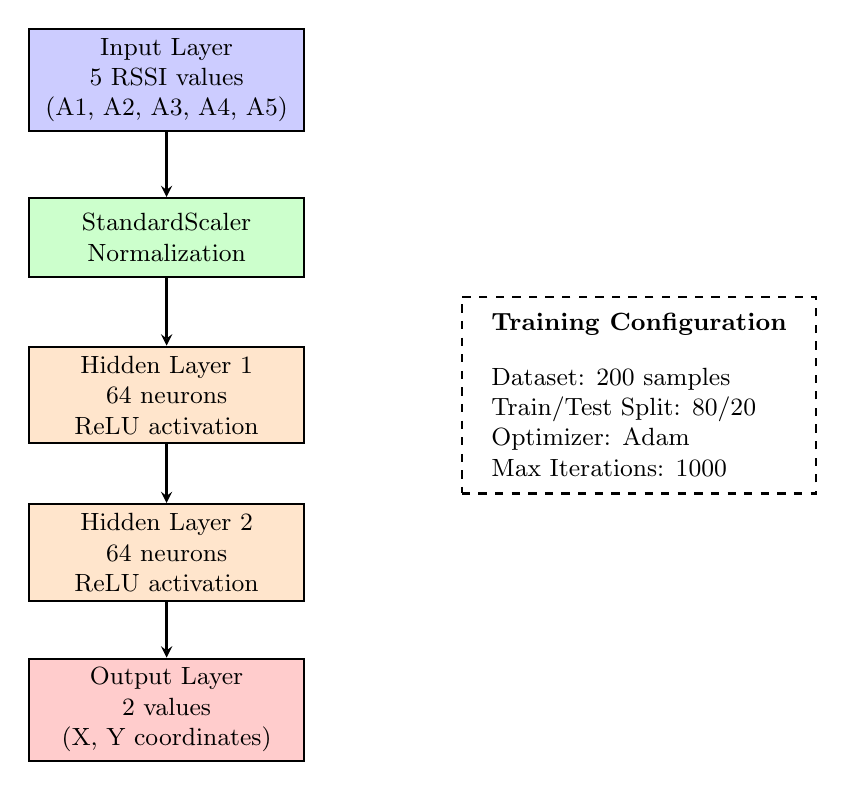
\begin{tikzpicture}[
    layer/.style={rectangle, draw, thick, minimum width=3.5cm, minimum height=1cm, align=center, font=\small},
    arrow/.style={->, >=stealth, thick}
]

% Input Layer
\node[layer, fill=blue!20] (input) at (0,0) {Input Layer\\5 RSSI values\\(A1, A2, A3, A4, A5)};

% StandardScaler
\node[layer, fill=green!20] (scaler) at (0,-2) {StandardScaler\\Normalization};

% Hidden Layer 1
\node[layer, fill=orange!20] (hidden1) at (0,-4) {Hidden Layer 1\\64 neurons\\ReLU activation};

% Hidden Layer 2
\node[layer, fill=orange!20] (hidden2) at (0,-6) {Hidden Layer 2\\64 neurons\\ReLU activation};

% Output Layer
\node[layer, fill=red!20] (output) at (0,-8) {Output Layer\\2 values\\(X, Y coordinates)};

% Arrows
\draw[arrow] (input) -- (scaler);
\draw[arrow] (scaler) -- (hidden1);
\draw[arrow] (hidden1) -- (hidden2);
\draw[arrow] (hidden2) -- (output);

% Training info box
\node[draw, dashed, thick, minimum width=4.5cm, minimum height=2.5cm, align=left, font=\small] (training) at (6,-4) {
    \textbf{Training Configuration}\\[0.3cm]
    Dataset: 200 samples\\
    Train/Test Split: 80/20\\
    Optimizer: Adam\\
    Max Iterations: 1000
};

\end{tikzpicture}